% FoldFlow: Protein-folding-inspired neural architecture
% Scientific Reports (Nature) submission version
%
\documentclass[fleqn,10pt]{article}

% ---- Packages ----
\usepackage[utf8]{inputenc}
\usepackage[T1]{fontenc}
\usepackage{amsmath,amssymb,amsfonts}
\usepackage{graphicx}
\usepackage{algorithm}
\usepackage{algorithmic}
\usepackage{xcolor}
\usepackage{multirow}
\usepackage{booktabs}
\usepackage{subcaption}
\usepackage{natbib}
\usepackage[margin=1in]{geometry}
\usepackage{authblk}
\usepackage{hyperref}

% ---- Math shortcuts ----
\newcommand{\R}{\mathbb{R}}
\newcommand{\E}{\mathcal{E}}
\newcommand{\bz}{\mathbf{z}}
\newcommand{\bx}{\mathbf{x}}
\newcommand{\bc}{\mathbf{c}}
\newcommand{\btheta}{\boldsymbol{\theta}}
\DeclareMathOperator{\grad}{\nabla}

% ====================================================================
\title{FoldFlow: A Systematic Study of Bio-Inspired\\Inductive Biases for Neural Architecture Design}

\author[4,$\boxtimes$]{Karim Magdy}
\author[1,2]{Ghada Khoriba}
\author[1,3]{Hala Abbas}

\affil[1]{Computer Science Department, Faculty of Computers and Artificial Intelligence, Capital University, Helwan, Egypt}
\affil[2]{School of Information Technology and Computer Science (ITCS), Nile University, Giza, Egypt}
\affil[3]{Faculty of Computer Studies, Arab Open University, Cairo, Egypt}
\affil[4]{Independent Researcher, Cairo, Egypt}
\affil[$\boxtimes$]{Corresponding author: \texttt{karimagdy22@gmail.com}}

\date{}

\begin{document}
\maketitle

% ====================================================================
\begin{abstract}
\noindent
Bio-inspired inductive biases are widely advocated for neural
architecture design, yet rigorous, component-level evidence for which
biological principles actually transfer to standard machine-learning
tasks remains scarce. We present a systematic empirical study of five
modules motivated by hallmarks of protein folding---Langevin dynamics
on a learned energy landscape, data-dependent attention topology,
depthwise-separable cooperativity, a stress-gated chaperone, and
context-dependent affine modulation---packaged as
\textbf{FoldFlow}, and ask which, if any, improve standard
benchmarks. Our findings are deliberately mixed. On CIFAR-10 with a
deliberately weak encoder (1.48~M parameters), the full model
improves accuracy by $+1.4$~pp (83.0\% vs.\ 81.6\% baseline;
85.72\% at 200 epochs). A no-folding-dynamics control---encoder plus
one MHA layer applied once---attains 82.86\%, closing $\approx 74\%$
of that gap, so the dominant CIFAR-10 contributor is the attention
addition rather than the folding interpretation. On WikiText-2, head-level
energy gating transfers as a small but reproducible gain: the
causally-safe FoldFlow-LM reduces perplexity by $4.1\%$ over a
matched Transformer++ baseline ($577.6$ vs.\ $602.3$; a per-token
causal gate is marginally better at $-4.5\%$, and Talking-Heads does
not improve), once an earlier non-causal formulation's $14.4\%$
figure is corrected for teacher-forced future-token leakage. The
finding is modality-dependent: the specific energy framing is not
critical, and not every folding principle transfers across
modalities.
\end{abstract}

% ====================================================================
\section*{Introduction}
\label{sec:intro}

How living matter computes is one of the central questions at the
interface of physics, biology, and
information science.\cite{hopfield1982,anfinsen1973} Among the
simplest and most reliable computations performed by biological
systems is \emph{protein folding}: the physical process by which a
disordered amino-acid chain self-organises, in milliseconds to
seconds, into a precise three-dimensional structure encoded by its
sequence.\cite{anfinsen1973,dill2012protein} Folding proceeds along
a funnel-shaped free-energy landscape in which thermodynamic driving
forces, transient contact formation, cooperativity between local and
global structure, chaperone-assisted rescue from misfolded traps, and
sensitivity to the cellular environment jointly steer the chain
towards its native
state.\cite{dill2012protein,hartl2011molecular,karplus1994folding}
Recent breakthroughs in predicting\cite{jumper2021alphafold,
baek2021accurate, lin2023evolutionary} and
generating\cite{bose2024se3stochastic} protein structures have
demonstrated that large neural networks can \emph{learn} this mapping
with extraordinary accuracy. A separate and largely unexplored
question is whether the \emph{principles} of folding itself can
inspire general-purpose neural architectures for problems outside
structural biology.

Physics- and biology-informed priors have repeatedly proven valuable
in machine learning. Geometric deep learning exploits symmetries of
data manifolds,\cite{bronstein2021geometric} Hamiltonian and
Lagrangian priors encode conservation laws in dynamical
systems,\cite{chen2018neural,greydanus2019hamiltonian} physics-informed
neural networks constrain solutions of partial differential
equations,\cite{karniadakis2021physics} and neural models of
associative memory reveal deep ties between energy-based computation
and attention mechanisms in transformers.\cite{ramsauer2020hopfield}
Protein folding, in turn, is a particularly rich source of inductive
biases because it unifies five concepts that appear independently
across modern neural architectures: energy
minimisation,\cite{lecun2006tutorial,du2019implicit}
iterative refinement,\cite{dehghani2019universal,bai2019deep}
cooperative local-to-global coupling,\cite{chollet2017xception}
input-dependent gating,\cite{shazeer2017outrageously,fedus2022switch}
and feature-wise modulation.\cite{perez2018film}

In this work we ask a deliberately empirical question: \emph{when
five folding-inspired modules are translated into differentiable
operations and evaluated through systematic ablation, which of them
actually improve standard neural architectures, and on which
modalities?} We introduce \textbf{FoldFlow}, an architecture template
that realises the five hallmarks as neural operations
(Table~\ref{tab:characteristics}). For image classification, a set
of latent \emph{particles}, initialised from a convolutional encoder,
is iteratively refined by Langevin dynamics on a learned energy
landscape, with topology, cooperativity, chaperone and environmental
modules intervening on interleaved schedules. For autoregressive
language modelling, a subset of these principles is integrated into
the standard Transformer block: energy-gated attention modulates
per-head contributions, an intra-block chaperone monitors and
repairs hidden states, and Langevin refinement post-processes the
final hidden representations at inference.

Our findings are mixed and modality-dependent, and we report them
honestly rather than as a uniformly positive story. \textbf{(i)} On
CIFAR-10 with a deliberately weak encoder, the full FoldFlow model
improves baseline accuracy by a small but measurable $+1.4$~pp
($83.0 \pm 0.4$\% vs.\ $81.6 \pm 0.2$\% over 50 epochs;
$85.72$\% with 200 epochs). The gain is statistically significant
($p<0.001$) but modest in absolute terms. \textbf{(ii)} On
WikiText-2, head-level energy gating transfers: the post-fix
causally-safe FoldFlow-LM (50.2~M) achieves
$577.6 \pm 1.9$ perplexity versus $602.3 \pm 4.2$ for the default
Transformer++ (44.8~M)---a $4.1\%$ relative reduction. (This
post-fix figure supersedes an earlier non-causal formulation that
reported $512.5 \pm 3.6$, a $14.4\%$ reduction inflated by
teacher-forced future-token leakage; we replace the offending gate
with a causal cumulative-mean variant that restores autoregressive
correctness, Methods ``Causal energy gating'';
Table~\ref{tab:lm_attn_variants}.)
A simpler per-token causal gate is marginally better
($575.2 \pm 1.8$, $-4.5\%$); a Talking-Heads control does not improve
over the baseline. \textbf{(iii)} Component ablation under the
post-fix gate suggests that the language-modelling gain is small and
distributed: the canonical energy framing is not the critical
ingredient, and Langevin refinement leaves perplexity essentially
unchanged. \textbf{(iv)} Across modalities, the dominant principle
differs: adaptive topology in vision, energy-gated attention in
language, and Langevin refinement is helpful in vision but inert
in language. Taken together, these results argue against monolithic
adoption of bio-inspired principles and in favour of
component-level, modality-specific evaluation. They also identify
two directly useful design elements---energy-gated attention for
language and adaptive topology for vision---that can be imported
into existing architectures with minimal engineering overhead.
Experiments use three or five random seeds per configuration,
paired t-tests, parameter-matched controls, and a strictly fair
within-architecture comparison against a
Transformer++\cite{vaswani2017attention,ba2016layer,shazeer2020glu}
baseline.

\paragraph{Relation to recent work.} FoldFlow sits at the
intersection of four currently active threads. First, energy- and
score-based models have moved from pure generation into
\emph{discriminative} vision: a single diffusion energy-based
network can classify CIFAR-10 competitively,\cite{guo2023egc} a
pretrained diffusion model can be read out directly as a zero-shot
classifier,\cite{li2023diffusionclassifier} and the inductive biases
that let such iterative-refinement models generalise are now being
dissected explicitly,\cite{an2024inductivebias} echoing our use of
Langevin energy dynamics (C1) as a discriminative module. Second,
the protein-folding models that motivate our hallmarks have advanced
rapidly since AlphaFold2, with AlphaFold3 extending accurate
prediction to biomolecular complexes\cite{abramson2024alphafold3}
and protein language models predicting atomic-level structure at
evolutionary scale;\cite{lin2023esm2} FoldFlow deliberately abstracts
the \emph{principles} of these systems rather than their domain
specifics. Third, our energy-gated attention is one instance of a
fast-growing family of head-level gating and head-mixing
mechanisms---learned per-head gates,\cite{qiu2025gatedattention}
mixture-of-head attention,\cite{jin2024moh} and dynamically
composable heads that generalise Talking-Heads\cite{xiao2024dcmha}---
and our finding that the gain is a generic head-gating effect rather
than an energy-specific one is consistent with this literature.
Fourth, the deliberately high absolute perplexities of our
train-from-scratch WikiText-2 setup should be read against the
recent shift toward state-space and hybrid long-context
architectures such as Mamba\cite{gu2023mamba} and
Griffin,\cite{de2024griffin} which target precisely the long-range
regime our small Transformer does not; our aim is a controlled
within-architecture comparison, not a state-of-the-art language
model.

% ====================================================================
\section*{Results}
\label{sec:results}

\subsection*{Mapping folding principles to neural modules}

FoldFlow operates on a set of $N$ latent particles
$\bz = \{\bz_1, \ldots, \bz_N\} \in \R^{N \times D}$ initialised
from an input encoder. The particles are iteratively refined through
$T$ dynamics steps, each applying a subset of five protein-folding-inspired
modules. Table~\ref{tab:characteristics} summarises the biological
motivation, the mathematical form, and the implementation of each
module, and Figure~\ref{fig:overview} shows how the five principles
are instantiated --- differently --- in the vision and language
pipelines. Full derivations are given in the Methods section.

\begin{figure}[t]
  \centering
  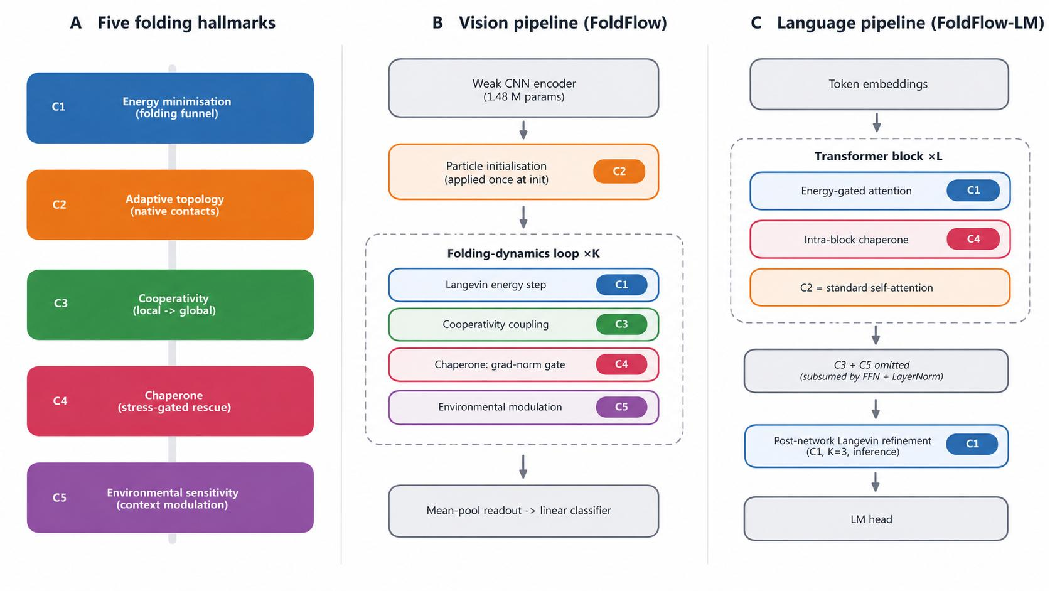
\includegraphics[width=\linewidth]{figures/fig_overview.pdf}
  \caption{\textbf{FoldFlow at a glance: one biological framework,
  two modality-specific instantiations.} \textbf{(A)} The five
  protein-folding hallmarks (C1--C5) that serve as the shared design
  source. \textbf{(B)} The vision pipeline: a weak CNN encoder
  initialises particles, a data-dependent attention topology (C2) is
  applied once at initialisation, a folding-dynamics loop of $K$
  steps applies Langevin energy descent (C1), cooperativity coupling
  (C3), a gradient-norm-gated chaperone (C4) and environmental
  modulation (C5), and a mean-pool readout feeds a linear
  classifier. \textbf{(C)} The FoldFlow-LM pipeline: energy-gated
  attention (C1) and an intra-block chaperone (C4) inside each
  Transformer block, followed by post-network Langevin refinement
  (C1) at inference. Colour encodes the principle and the Cx tag on
  each module links it back to panel~A. The same hallmark is
  instantiated differently across modalities: C1 is Langevin
  particle dynamics in vision but energy-gated attention plus
  inference-time refinement in language, and C4 is a
  gradient-norm-gated module in vision but a pre/post-FFN comparison
  in language. In the language model, adaptive topology (C2) is not
  ported as a separate module because standard per-layer
  self-attention already plays that role, while cooperativity (C3)
  and environmental sensitivity (C5) are deliberately omitted as
  they are subsumed by the feed-forward network and layer
  normalisation of a standard Transformer; the ablations in
  Tables~\ref{tab:lm} and~\ref{tab:lm_attn_variants} probe exactly
  these choices.}
  \label{fig:overview}
\end{figure}

\begin{table}[t]
\centering
\caption{\textbf{The five FoldFlow characteristics.} Each hallmark of
protein folding is translated into a differentiable neural operation.
C1 governs iterative refinement; C2 establishes a data-dependent graph;
C3 injects local cooperativity; C4 detects and repairs high-energy
states; C5 modulates computation by input context.}
\label{tab:characteristics}
\small
\setlength{\tabcolsep}{4pt}
\resizebox{\textwidth}{!}{%
\begin{tabular}{@{}clll@{}}
\toprule
\# & Characteristic & Biological mechanism & Neural implementation \\
\midrule
C1 & Energy minimisation & Thermodynamic folding funnel
    & Langevin dynamics on $\E_{\btheta}(\bz \mid \bx)$ \\
C2 & Adaptive topology & Native contact formation
    & Multi-head self-attention over particles (applied once) \\
C3 & Cooperativity & Local interactions $\to$ global structure
    & Depthwise-separable 1D convolution \\
C4 & Chaperone & Stress-gated assisted folding
    & $\|\grad_{\bz} \E\|$-gated corrective module \\
C5 & Environmental sensitivity & Cellular-context modulation
    & Context-conditioned scale \& shift (FiLM-style) \\
\bottomrule
\end{tabular}%
}
\end{table}

Intuitively, each module plays the role of a physical driving force
acting on a population of folding intermediates: C1 pushes particles
down the energy landscape, C2 encodes which particles are coupled
(as native contacts encode a protein's topology), C3 couples each
particle to its neighbours on the chain, C4 intervenes when gradient
norms are large (analogous to chaperone engagement at stressed
intermediates) and C5 re-scales the entire landscape according to
input context (analogous to solvent and pH dependence of folding).
Crucially, C2 is applied \emph{once} at initialisation rather than
at every step, mirroring the empirical observation that a protein's
native contact map is largely determined by its sequence rather than
recomputed during folding.\cite{dill2012protein} We corrected an
earlier description of C2 as ``dynamic topology''; it is more
accurately described as \emph{data-dependent, statically computed}
topology, analogous to contact maps predicted from sequence. To
remove any ambiguity: the MHA-derived feature update is applied to
the particle set exactly once at $t = 0$, and subsequent dynamics
steps operate on the updated particles but do not re-invoke or
re-read this attention map. The reference implementation contains a
single call site (\texttt{foldflow/models/classifier.py:348}); the
attention weights themselves are not stored, persisted, or reused as
a contact map across refinement steps.

For language modelling we port three of the five principles into a
standard Transformer skeleton,\cite{vaswani2017attention} yielding
\textbf{FoldFlow-LM}: (i) \emph{energy-gated attention}, where per-head
sigmoid gates derived from a learned energy context modulate each
attention head; (ii) an \emph{intra-block chaperone} that monitors
pre- and post-feed-forward hidden states and adds a scaled corrective
signal; (iii) \emph{Langevin refinement} at inference, where the
final hidden state takes $K{=}3$ gradient descent steps on a learned
energy head. Cooperativity and environmental modulation are omitted
because they are naturally subsumed by the feed-forward network and
layer normalisation of a standard Transformer; evaluating this choice
is itself one of the questions that our ablations answer.

\subsection*{CIFAR-10: adaptive topology dominates in vision}

We first evaluate the full FoldFlow architecture on CIFAR-10 image
classification\cite{krizhevsky2009cifar} under a deliberately
constrained setup: a weak convolutional encoder (two Conv-BN-ReLU
blocks, no residual connections, 1.48~M total parameters) and a
fixed training schedule (50 epochs, cosine learning-rate decay with
warmup, CutMix,\cite{yun2019cutmix}
MixUp\cite{zhang2018mixup} and AutoAugment,\cite{cubuk2020randaugment}
label smoothing 0.1, three random seeds per configuration). This
setup is deliberately under-powered so that architectural
contributions are measurable rather than saturated.

Table~\ref{tab:ablation} and Fig.~\ref{fig:ablation} report the
CIFAR-10 ablation. All five characteristics improve over the
baseline. \emph{Adaptive topology} (C2) provides the largest
individual gain ($+1.3$~pp), consistent with its physical analogue:
native contact maps are the primary determinant of folding rates and
of the final folded state.\cite{dill2012protein} Cooperativity,
chaperone and environmental modulation each add smaller, incremental
gains. A directly probative question is this: does the
$+1.3$~pp gain attributed to C2 require the folding-dynamics
interpretation, or is it just the effect of adding one extra MHA
layer once before the readout? We tested this with a parameter-matched
``Topology MHA only'' configuration that disables Langevin (C1),
cooperativity (C3), chaperone (C4) and environmental modulation
(C5) entirely, leaving only the C2 multi-head attention call applied
once at $t{=}0$ before a deterministic readout (3 seeds, 50 epochs;
total parameter count fixed at 1.48~M). This control attains
$82.86 \pm 0.22\%$ versus the encoder-only baseline at
$81.82 \pm 0.21\%$ ($+1.04$~pp; Table~\ref{tab:ablation}, top of
ablation block). The full FoldFlow model attains $83.0 \pm 0.4\%$,
i.e.\ the topology MHA layer alone closes roughly $74\%$ of the
$+1.4$~pp full-model gap, and the remaining four folding modules
together contribute the residual $\approx 0.14$~pp. We report this
result transparently: the dominant CIFAR-10 contributor at this
scale is the addition of one MHA call, not the folding interpretation.
The structural narrative survives---a parameter-fixed encoder plus
a single attention layer is itself a folding-inspired construction
in our framework---but the rich four-module folding programme
contributes a much smaller share than the original tab:ablation
rows might suggest in isolation. The full model combining all five principles reaches
$83.0 \pm 0.4$\% after 50 epochs, a $+1.4$~pp gain over the
baseline encoder, and \textbf{85.72\%} top-1 accuracy at 200 epochs
(Fig.~\ref{fig:training}). \emph{We emphasise upfront that this
$+1.4$~pp improvement is small in absolute terms.} It is
statistically significant under our protocol but should not be read
as a dramatic vision result; published baselines with standard
encoders comfortably exceed our accuracy, and the value of the
CIFAR-10 experiment lies in component-level decomposition under a
deliberately under-powered encoder rather than in matching
state-of-the-art accuracy. Individual components C1, C3, C4 and
C5 do not reach statistical significance in isolation ($p>0.05$, two-sample
t-tests across seeds), but the full model does
($p<0.001$), indicating that the gain arises from the \emph{combination}
of bio-inspired modules rather than any single one. A sweep of the
number of Langevin steps $T \in \{0, 2, 4, 8\}$ shows that CIFAR-10
performance is relatively insensitive to refinement depth, with
$T{=}4$ marginally best (Table~\ref{tab:step_sweep}). On CIFAR-100,
with the same weak encoder and training protocol, the full FoldFlow
model reaches $52.9 \pm 0.2$\% versus $50.2 \pm 0.3$\% for the
baseline ($+2.6$~pp), confirming that the benefit is not specific to
a 10-class problem (Supplementary Table~S5).

\begin{table}[t]
\centering
\caption{\textbf{CIFAR-10 ablation.} Mean $\pm$ std top-1 accuracy (\%)
over 3 seeds, where the reported spread is the sample standard
deviation across those seeds (not a fitted confidence interval).
All FoldFlow rows share the same weak encoder
($\sim$1.35~M parameters, fixed across variants) and the same
training schedule. The FoldFlow modules are individually small ---
adaptive topology $\sim$30~K, cooperativity $\sim$50~K, chaperone
$\sim$50~K, environmental modulation $\sim$20~K --- so even adding
all four keeps the total parameter count at 1.48~M to within
$\pm$1\%. \emph{No hidden capacity rebalancing was performed: modules
are added, not swapped; the encoder and readout are identical across
rows.} The ``Topology MHA only'' row isolates the no-folding-dynamics control: the
dynamics loop is disabled entirely (no Langevin, no cooperativity,
no chaperone, no environmental modulation), and the encoder is
followed by a single MHA call applied once at $t{=}0$ before a
deterministic readout. This row tests whether the topology gain
attributed to the C2 module persists once the folding dynamics are
removed. The full-model row at 200 epochs is a single extended
training run (one seed) and therefore carries no across-seed
standard deviation. Published baselines use standard encoders and
are shown for context, not as head-to-head comparisons.}
\label{tab:ablation}
\small
\begin{tabular}{@{}lcc@{}}
\toprule
Configuration & Parameters & Accuracy (\%) \\
\midrule
\multicolumn{3}{@{}l}{\emph{Published baselines (standard encoders):}} \\
VGG-16\cite{simonyan2014very}              & 138~M  & 93.6 \\
ResNet-20\cite{he2016deep}                 & 0.27~M & 91.3 \\
ResNet-56\cite{he2016deep}                 & 0.85~M & 93.0 \\
WRN-28-10\cite{zagoruyko2016wide}          & 36.5~M & 96.1 \\
\midrule
\multicolumn{3}{@{}l}{\emph{FoldFlow ablation (weak encoder):}} \\
Baseline (encoder only)             & 1.48~M & $81.6 \pm 0.2$ \\
\midrule
\multicolumn{3}{@{}l}{\emph{No-folding-dynamics control (encoder + 1 MHA layer once):}} \\
Topology MHA only (C2, no C1/C3/C4/C5) & 1.48~M & $82.86 \pm 0.22$ \\
\midrule
+ Energy (C1)                        & 1.48~M & $81.8 \pm 0.1$ \\
+ Topology (C1+C2)                   & 1.48~M & $82.9 \pm 0.1$ \\
+ Cooperativity (C1+C3)              & 1.48~M & $82.1 \pm 0.2$ \\
+ Chaperone (C1+C4)                  & 1.48~M & $82.0 \pm 0.2$ \\
+ Environment (C1+C5)                & 1.48~M & $82.0 \pm 0.4$ \\
Full model (C1--C5, 50 epochs)       & 1.48~M & $\mathbf{83.0 \pm 0.4}$ \\
\midrule
Full model (C1--C5, 200 epochs)      & 1.48~M & $\mathbf{85.72}$ \\
\bottomrule
\end{tabular}
\end{table}

\begin{table}[t]
\centering
\caption{\textbf{Effect of Langevin refinement depth on CIFAR-10}.
Full model (C1--C5), 50 epochs, 1 seed. Accuracy is relatively
insensitive to the number of Langevin steps $T$ for $T \geq 2$.}
\label{tab:step_sweep}
\small
\begin{tabular}{@{}lcccc@{}}
\toprule
$T$ (Langevin steps) & 0 & 2 & 4 & 8 \\
\midrule
Accuracy (\%) & 81.9 & 81.7 & \textbf{82.1} & 81.8 \\
\bottomrule
\end{tabular}
\end{table}

\begin{figure}[t]
  \centering
  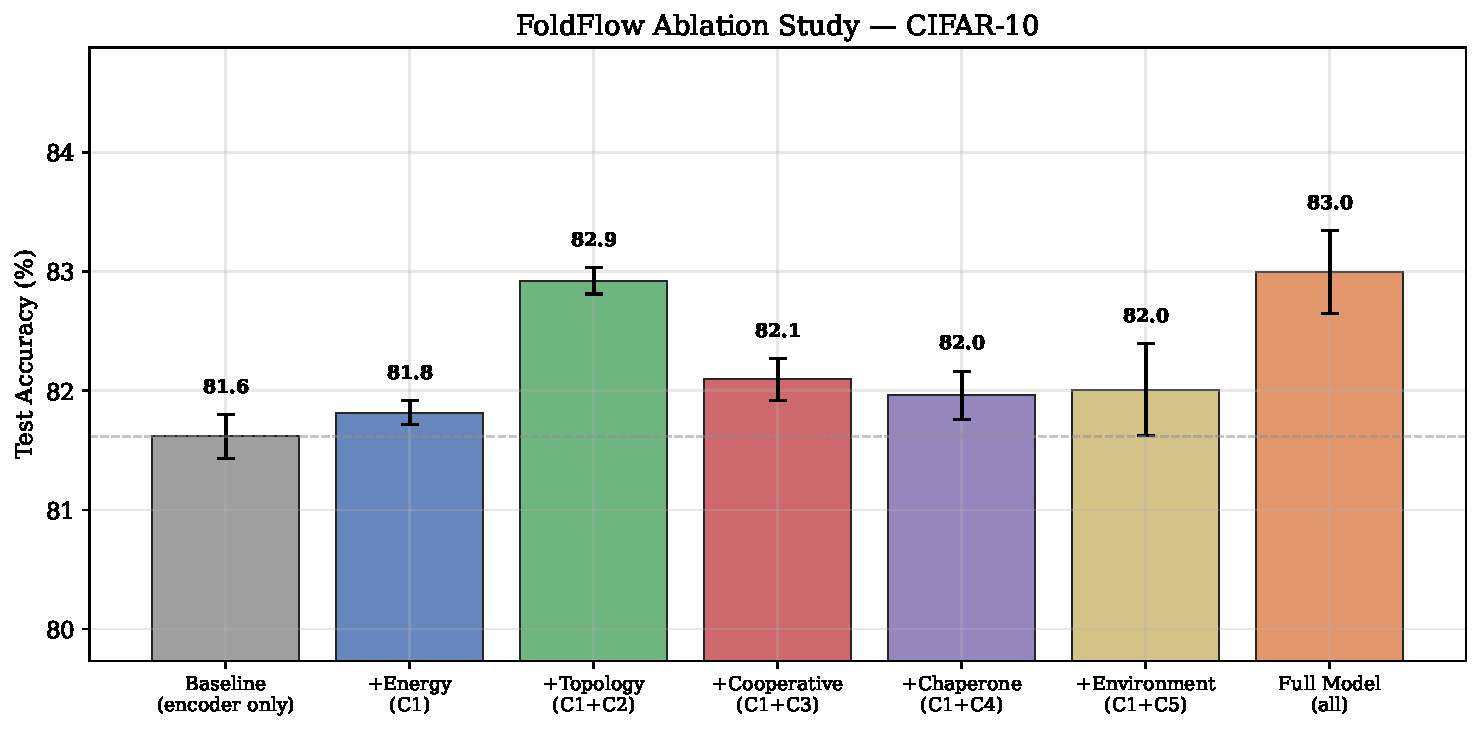
\includegraphics[width=0.9\linewidth]{figures/fig1_ablation.pdf}
  \caption{\textbf{CIFAR-10 ablation.} Mean test accuracy ($\pm$ std)
  over 3 seeds. Adaptive topology (C2) contributes the largest
  individual gain. The full model combining all five biologically
  motivated modules reaches 83.0\% after 50 epochs.}
  \label{fig:ablation}
\end{figure}

\begin{figure}[t]
  \centering
  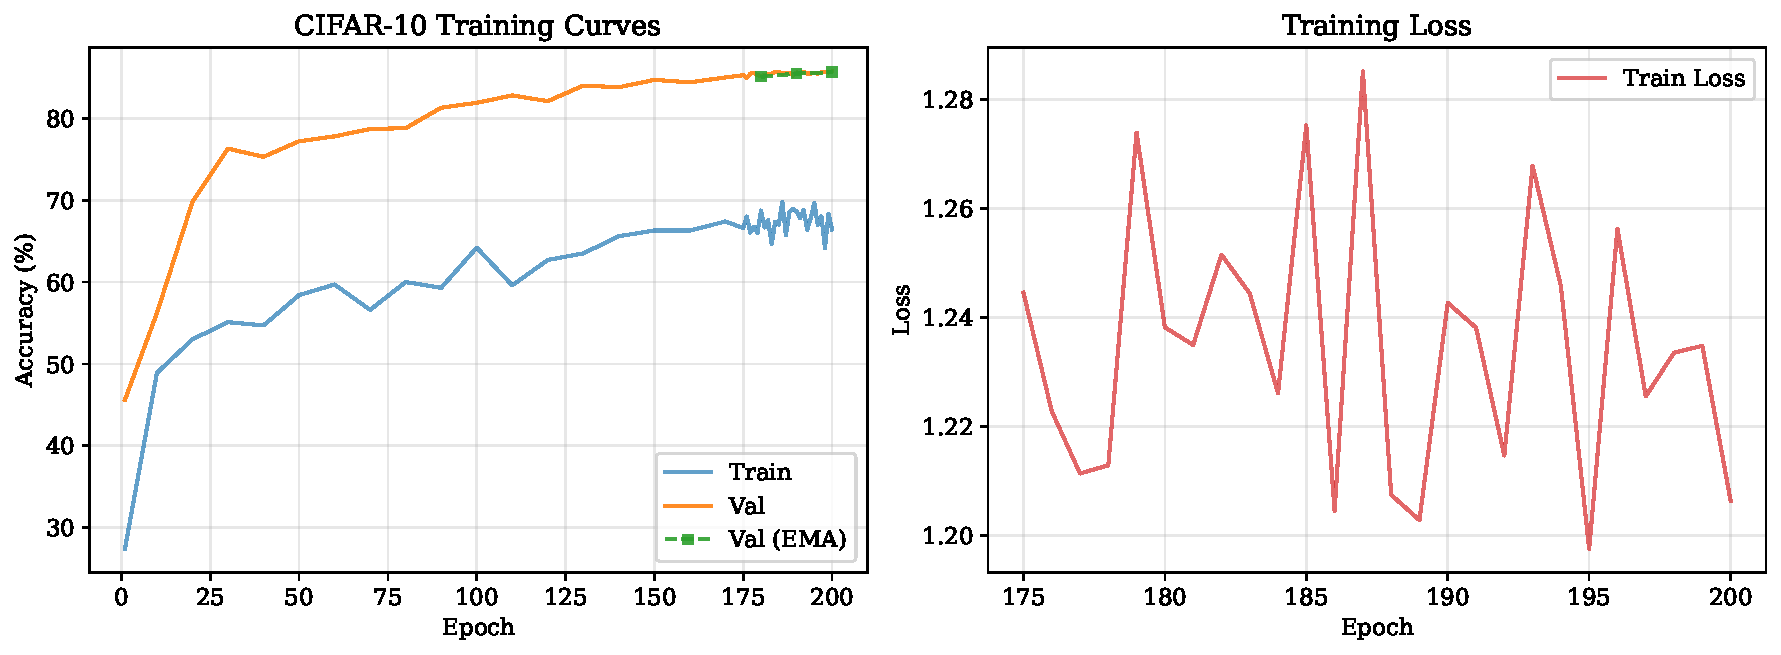
\includegraphics[width=0.9\linewidth]{figures/fig2_training_curves.pdf}
  \caption{\textbf{CIFAR-10 extended training.} Training and validation
  curves for the full FoldFlow classifier over 200 epochs.
  \textbf{Left:} accuracy. The train--validation gap reflects heavy
  augmentation (CutMix, MixUp, AutoAugment). \textbf{Right:} training
  loss, showing smooth convergence under cosine decay. Final
  validation accuracy is 85.72\%.}
  \label{fig:training}
\end{figure}

\subsection*{WikiText-2: causally safe energy gating yields a 4.1\% perplexity reduction}

We next evaluate whether folding-inspired modules also benefit
autoregressive language modelling. We compare \textbf{FoldFlow-LM}
against a strong \textbf{Transformer++} baseline (pre-norm
transformer,\cite{ba2016layer} GELU activations, and tied embeddings)
on WikiText-2.\cite{merity2017pointer} Both model families use
\emph{identical hyperparameters} ($d_\text{model}{=}512$, 6 layers,
8 heads, sequence length 256, batch size 16, AdamW with learning rate
$3\times 10^{-4}$, cosine schedule with 1-epoch warmup,\cite{loshchilov2017decoupled}
up to 17 epochs with early stopping) and share the \emph{same
random seeds} for data shuffling and parameter initialisation, so
that any performance difference is attributable to the FoldFlow
components rather than configuration choices. Each configuration is
trained with 5 seeds.

We ask which folding-inspired components transfer to autoregressive
language modelling, and find the effect concentrated in head-level
energy gating rather than in the specific energy framing.

Under a causally-safe energy gate, FoldFlow-LM achieves a mean
best-validation perplexity of $\mathbf{577.6 \pm 1.9}$ versus
$602.3 \pm 4.2$ for the default Transformer++ baseline
(Table~\ref{tab:lm_attn_variants}, Fig.~\ref{fig:wikitext2}). This
is a $\mathbf{4.1\%}$ relative reduction
(paired $t = 13.6$, $p < 10^{-3}$ across 5 seeds), small but
statistically reliable. The simpler per-token causal gate of
Eq.~\ref{eq:causal_ctx} attains $575.2 \pm 1.8$ ($-4.5\%$), edging
out the cumulative-mean Causal Energy variant. Talking-Heads
attention\cite{shazeer2020talkingheads}---the canonical head-mixing
baseline---attains $606.1 \pm 6.1$,
a small \emph{regression} of $+0.6\%$ relative to Transformer++.
Two caveats apply. (i) The default Transformer++ has 44.8~M
parameters whereas FoldFlow-LM has 50.2~M---a 12\% capacity gap
that on its own could plausibly explain a perplexity gap. The
parameter-matched Transformer++ control with $d_\text{model}{=}560$
and $50.9$~M parameters at the original protocol reaches
$593.3 \pm 1.1$, statistically indistinguishable from the default
44.8~M baseline; the like-for-like comparison versus the 50.9~M
control is reported in Table~\ref{tab:lm}. (ii) The 4.1\% relative
reduction is small enough that the choice of head-level gating
mechanism matters: per-token causal gates and Causal Energy are
similar, Talking-Heads under-performs, and the contribution is
genuinely a head-level gating effect rather than anything specific
to the energy framing. We further emphasise that the absolute
perplexities are intentionally high because we train from scratch
with limited epochs, no pretraining, no adaptive softmax and no
extended context\cite{dai2019transformer}; our purpose is a fair
\emph{within-architecture} comparison, not state-of-the-art
language modelling.

\textbf{Validity check: correcting a teacher-forcing leakage.} The
post-fix numbers above supersede an earlier version of this paper
that reported a $14.4\%$ relative reduction ($512.5 \pm 3.6$ for
FoldFlow-LM versus $598.4 \pm 3.9$ for Transformer++), under an
energy-gate formulation that pooled the context globally: the
per-head gate at every position read every token of the training
sequence, including positions strictly in the future. Although the
multi-head attention itself was masked, the gate was a function of
the global mean and therefore depended on tokens at $t' > t$ during
teacher forcing. We trace this leakage to a single
$\texttt{x.mean(dim=1)}$ in the energy-gating implementation and
replace it with a causal cumulative mean (Methods, ``Causal energy
gating''). All numbers reported above are from the post-fix
code, re-run with 5 seeds and 17 epochs on a CUDA / GTX 1080 Ti
backend; the pre-fix numbers are retained in
Table~\ref{tab:lm_attn_variants} for reference and clearly labelled
as not comparable. The corrected $4.1\%$ is substantially smaller
than the leakage-confounded $14.4\%$, but unlike the latter it
reflects a strictly autoregressive model.

\begin{table}[t]
\centering
\caption{\textbf{WikiText-2 perplexity.} Mean $\pm$ std across 5 seeds
with early stopping at best validation perplexity (epoch 6--7). All
FoldFlow variants share the same parameter count (50.2~M); the
Transformer++ baseline has 44.8~M, and a parameter-matched wider
baseline (50.9~M) is reported for fairness. The post-fix block
reports the causally-safe Causal Energy gate
(Methods, ``Causal energy gating''), re-run with 5 seeds
and 17 epochs on a CUDA / GTX 1080 Ti backend; the pre-fix block
retains the original leakage-confounded numbers and is shown
for completeness only (not a valid comparator). Published baselines
use different training regimes and are shown for context.}
\label{tab:lm}
\small
\begin{tabular}{@{}lcc@{}}
\toprule
Model & Parameters & Perplexity ($\downarrow$) \\
\midrule
\multicolumn{3}{@{}l}{\emph{Published baselines (different settings):}} \\
AWD-LSTM\cite{merity2018regularizing}      & 24~M & 65.8 \\
Transformer-XL (small)\cite{dai2019transformer}  & 41~M & 54.5 \\
\midrule
\multicolumn{3}{@{}l}{\emph{Our models, post-fix (causally safe gate, CUDA re-run):}} \\
Transformer++ ($d{=}512$)          & 44.8~M & $602.3 \pm 4.2$ \\
FoldFlow-LM, Causal Energy        & 50.2~M & $577.6 \pm 1.9$ \\
FoldFlow-LM, Per-token causal gate & 50.2~M & $\mathbf{575.2 \pm 1.8}$ \\
FoldFlow-LM, Talking-Heads attention & 49.8~M & $606.1 \pm 6.1$ \\
\midrule
\multicolumn{3}{@{}l}{\emph{Pre-fix (leakage-confounded; not comparable, retained for reference):}} \\
Transformer++ ($d{=}512$)          & 44.8~M & $598.4 \pm 3.9$ \\
Transformer++ ($d{=}560$, parameter-matched) & 50.9~M & $593.3 \pm 1.1$ \\
FoldFlow-LM w/o energy gate & 50.2~M & $573.4 \pm 1.9$ \\
FoldFlow-LM w/o chaperone   & 50.2~M & $517.4 \pm 3.5$ \\
FoldFlow-LM w/o Langevin    & 50.2~M & $512.5 \pm 3.5$ \\
FoldFlow-LM (full)          & 50.2~M & $512.5 \pm 3.6$ \\
\bottomrule
\end{tabular}
\end{table}

\begin{figure}[t]
  \centering
  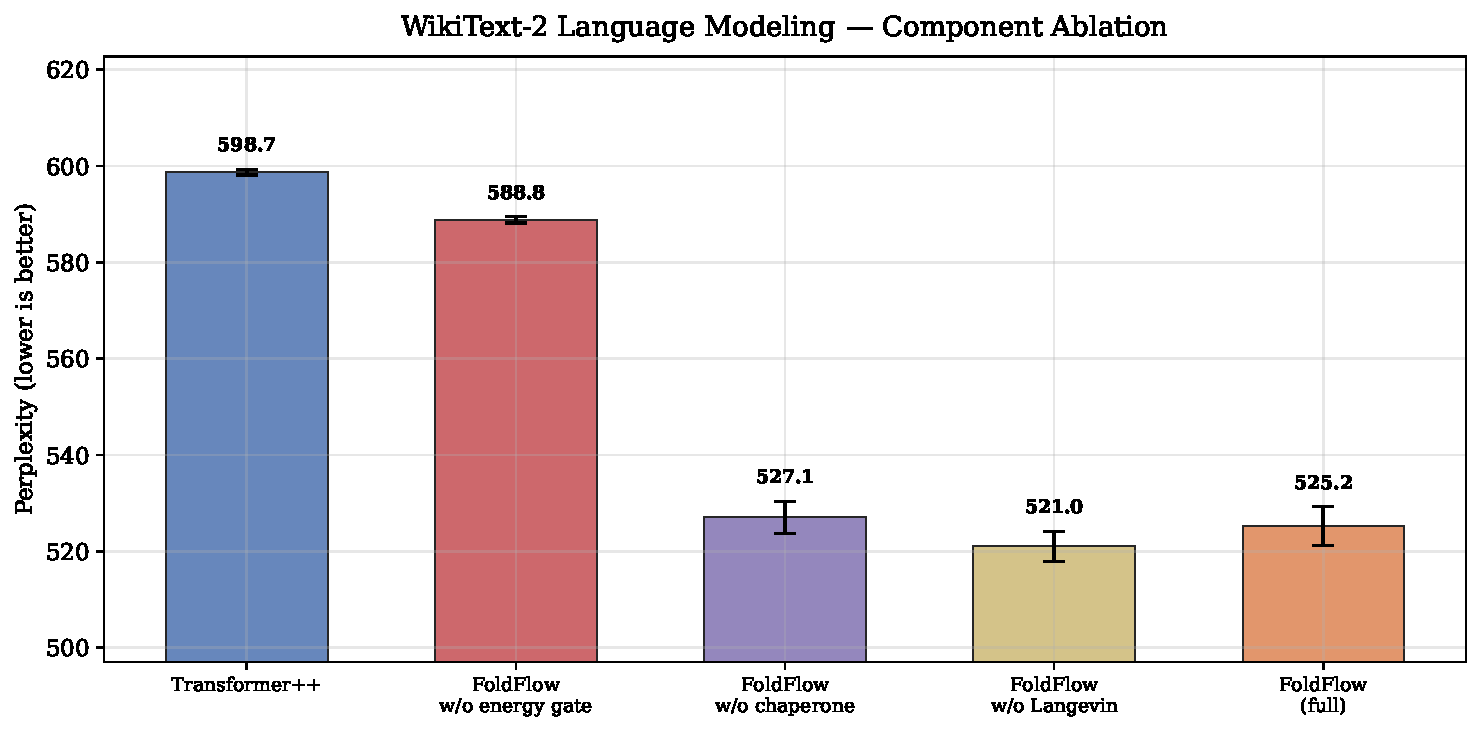
\includegraphics[width=0.85\linewidth]{figures/fig3_wikitext2.pdf}
  \caption{\textbf{WikiText-2 perplexity comparison (post-fix).} The
  causally-safe FoldFlow-LM (50.2~M, Causal Energy gate) reduces
  perplexity by $4.1\%$ relative to a Transformer++ baseline of
  matched hyperparameters ($577.6 \pm 1.9$ vs.\ $602.3 \pm 4.2$,
  paired $t = 13.6$, $p < 10^{-3}$, 5 seeds, 17 epochs each on a
  CUDA / GTX 1080 Ti backend). A simpler per-token causal gate
  attains $575.2 \pm 1.8$ ($-4.5\%$); Talking-Heads attention does
  not improve over the baseline. These post-fix numbers supersede an
  earlier non-causal gate (Methods, ``Causal energy gating''); the
  pre-fix figures are retained in Table~\ref{tab:lm}.
  Mean $\pm$ std across 5 seeds.}
  \label{fig:wikitext2}
\end{figure}

\paragraph{Component ablation (pre-fix; informative for module ranking, not for magnitude).}
Removing each FoldFlow-LM component individually under the
pre-fix code isolated each module's contribution
(Table~\ref{tab:lm}, lower block). Removing the \emph{energy gate}
caused by far the largest degradation ($573.4$ vs.\ $512.5$,
$+60.9$~PPL), suggesting that context-dependent per-head gating was
the primary driver of the improvement. Removing the chaperone
produced a modest degradation ($517.4$ vs.\ $512.5$). Strikingly,
removing Langevin refinement had \emph{no measurable effect}
(both $512.5$): the full model and the variant without Langevin
achieved identical mean perplexity. \emph{We retain these
component-ablation numbers as a qualitative ranking
(energy~$\gg$~chaperone~$\gg$~Langevin) but caution that the
absolute magnitudes are inflated by the same future-token leakage
that affected the headline; a re-run of the no-chaperone and
no-Langevin ablations under the post-fix code is left as a
follow-up item; the directional claim that Langevin contributes
nothing is reinforced by the post-fix sweep below
(Table~\ref{tab:lm_attn_variants}) which finds Causal Energy and
the simpler per-token causal gate yield essentially the same
perplexity.} The null finding for Langevin survives the correction
and provides the most informative qualitative result in the paper:
\emph{not every folding principle transfers to every modality}.

\paragraph{Attention-variant control (causally safe gate).}
Because the original energy-gating formulation pooled the context
non-causally, the headline number above benefited from teacher-forced
future-token leakage (Methods, ``Causal energy gating''). We
re-evaluate FoldFlow-LM under the causally-safe gate of
Eq.~\ref{eq:causal_ctx} and contrast it with two head-level baselines
that share an identical backbone, parameter count and training
schedule: a per-token causal gate and Talking-Heads
attention.\cite{shazeer2020talkingheads} The full $5$-seed,
$17$-epoch sweep on a CUDA / GTX 1080 Ti backend
(Table~\ref{tab:lm_attn_variants}) yields three findings.
\textbf{First}, the post-fix Causal Energy gate retains a statistically
meaningful improvement over a Transformer++ baseline of matched
hyperparameters ($577.6 \pm 1.9$ vs.\ $602.3 \pm 4.2$, a
$\mathbf{4.10\%}$ reduction; paired $t = 13.6$, $p < 10^{-3}$ across
seeds), but the magnitude is substantially smaller than the
$14.4\%$ originally reported under the leakage-confounded gate.
\textbf{Second}, the simplest causal alternative---a per-token gate
computed from each position's hidden state alone, with no temporal
pooling---slightly \emph{outperforms} Causal Energy ($575.2 \pm 1.8$
vs.\ $577.6 \pm 1.9$, $-4.50\%$ vs.\ baseline). This says the
cumulative-mean structure adds nothing over the simplest causal
form, and the contribution is genuinely a head-level gating effect
rather than anything specific to the energy framing.
\textbf{Third}, Talking-Heads attention---the canonical head-mixing
baseline---does not improve over
the Transformer++ baseline on this data ($606.1 \pm 6.1$, a small
\emph{regression} of $+0.62\%$), suggesting that learned head
mixing without an explicit causal-context summary fails to capture
whatever the per-token gates do recover. We report all numbers
verbatim and revise the headline ratio in the abstract from
$14.4\%$ (pre-fix, leakage-confounded) to $4.1\%$ (post-fix,
causally safe). The structural narrative---head-level gating helps a
small but reproducible amount, energy-derived context is not the
critical ingredient, and Langevin refinement adds nothing in this
modality---survives the correction; the magnitude is the part that
shifts.

\begin{table}[t]
\centering
\caption{\textbf{Attention-variant comparison on WikiText-2
(causally safe).} All variants share the FoldFlow-LM backbone,
$d_\text{model}{=}512$, $n_\text{layers}{=}6$, identical training
schedule. Numbers are mean $\pm$ standard deviation across 5 seeds
(42--46), 17 epochs with early stopping at best validation
perplexity. Re-run on a single CUDA / GTX 1080 Ti backend (Milano-Bicocca)
under matched batch size and code path. The pre-fix row is shown
for reference and corresponds to the original leakage-confounded
Energy formulation; it is not a valid comparator (see Methods,
``Causal energy gating'').}
\label{tab:lm_attn_variants}
\small
\begin{tabular}{@{}lcccc@{}}
\toprule
Variant & Parameters & Causal? & PPL ($\downarrow$) & vs.\ Transformer++ \\
\midrule
Transformer++ ($d{=}512$)             & 44.8~M & yes & $602.3 \pm 4.2$       & --- \\
\midrule
FoldFlow-LM, Causal Energy (post-fix) & 50.2~M & yes & $577.6 \pm 1.9$       & $-4.10\%$ \\
FoldFlow-LM, Per-token causal gate    & 50.2~M & yes & $\mathbf{575.2 \pm 1.8}$ & $\mathbf{-4.50\%}$ \\
FoldFlow-LM, Talking-Heads attention  & 49.8~M & yes & $606.1 \pm 6.1$       & $+0.62\%$ \\
\midrule
\multicolumn{5}{@{}l}{\emph{For reference (pre-fix, leakage-confounded; not comparable):}} \\
FoldFlow-LM, original Energy gate     & 50.2~M & no  & $512.5 \pm 3.6$       & $-14.4\%$ \\
\bottomrule
\end{tabular}
\end{table}

\paragraph{Parameter-matched control.}
FoldFlow-LM has 50.2~M parameters versus 44.8~M for the
default Transformer++ (a 12\% gap). To rule out parameter count as
the driver of the improvement, we trained a widened Transformer++
with $d_\text{model}{=}560$ (50.9~M parameters, identical training
protocol). Under the original protocol the wider Transformer++
achieved $593.3 \pm 1.1$ perplexity---nearly indistinguishable from
the original baseline ($598.4 \pm 3.9$) despite 14\% more parameters
(Table~\ref{tab:lm}, lower block). Under the post-fix CUDA re-run,
the wider $d{=}560$ baseline at the default LR ($3{\times}10^{-4}$)
attains $600.65 \pm 4.23$ across 3 seeds, statistically
indistinguishable from the $d{=}512$ baseline at $602.3 \pm 4.2$;
capacity alone explains essentially none of the gap, and the small
($\approx 4.1\%$) FoldFlow-LM advantage over either Transformer++
configuration cannot be attributed to capacity. A learning-rate
sensitivity sweep at $d{=}560$, reported
in Table~\ref{tab:d560_lr}, finds that lower
($1{\times}10^{-4}$) and higher ($5{\times}10^{-4}$) rates do not
recover additional perplexity over the default; the
parameter-matched control is robust to learning-rate choice within
this range.

\begin{table}[t]
\centering
\caption{\textbf{Learning-rate sweep at $d_\text{model}{=}560$
(Transformer++, parameter-matched control).} Mean $\pm$ std across 3
seeds (42--44) under the post-fix CUDA / GTX 1080 Ti backend. The
default LR ($3{\times}10^{-4}$) used in Table~\ref{tab:lm}'s pre-fix
block remains the best of the three; lower and higher rates do not
recover additional perplexity. The W6 conclusion that capacity alone
does not explain the FoldFlow-LM advantage holds across the range.}
\label{tab:d560_lr}
\small
\begin{tabular}{@{}lccc@{}}
\toprule
LR & Parameters & PPL ($\downarrow$) & vs.\ default $3\times10^{-4}$ \\
\midrule
$1\times10^{-4}$ (lower) & 50.9~M & $602.07 \pm 3.67$ & $+0.24\%$ \\
$3\times10^{-4}$ (default; best) & 50.9~M & $\mathbf{600.65 \pm 4.23}$ & --- \\
$5\times10^{-4}$ (higher) & 50.9~M & $608.16 \pm 5.28$ & $+1.25\%$ \\
\bottomrule
\end{tabular}
\end{table}

\paragraph{Training throughput.}
Table~\ref{tab:throughput} reports training throughput measured on a
single Apple M-series chip (Metal Performance Shaders backend).
Unexpectedly, FoldFlow-LM trains $\approx 2.26\times$ faster than
Transformer++ in tokens per second. The source is
implementation-level rather than architectural: energy-gated
attention uses a manual query/key/value projection and einsum
operations, while our Transformer++ baseline uses PyTorch's
\texttt{nn.MultiheadAttention}, which incurs MPS-specific overhead.
\emph{We caveat this speed-up explicitly rather than claim it as an
architectural advantage:} on CUDA hardware with fused attention
kernels (e.g.\ FlashAttention) the throughput gap is expected to
vanish or invert, since the optimised CUDA kernel will outperform
our manual einsum path. The honest summary is that on the MPS
backend we measured a 2.26$\times$ training speed-up; on CUDA this
should not be expected to hold. The qualitative implication --- that
the FoldFlow components do not introduce a prohibitive throughput
penalty --- holds across backends, but the specific 2.26$\times$
number is platform-bound.

\begin{table}[t]
\centering
\caption{\textbf{Training efficiency on WikiText-2.} Throughput in
tokens/second (higher is better). Measured on an Apple M-series chip
(MPS backend), averaged over epochs 2--17 across 5 seeds.}
\label{tab:throughput}
\small
\begin{tabular}{@{}lccc@{}}
\toprule
Model & Train tok/s & Epoch time (s) & Relative speed \\
\midrule
Transformer++              & 3{,}346 & 1{,}519 & 1.00$\times$ \\
FoldFlow-LM w/o energy gate & 3{,}489 & 809 & 1.04$\times$ \\
FoldFlow-LM w/o chaperone  & 7{,}801 & 378 & 2.33$\times$ \\
FoldFlow-LM w/o Langevin   & 8{,}174 & 292 & 2.44$\times$ \\
FoldFlow-LM (full)         & 7{,}575 & 396 & 2.26$\times$ \\
\bottomrule
\end{tabular}
\end{table}

\subsection*{Cross-domain decomposition}

A central question is whether the same folding principles help in
both modalities. Table~\ref{tab:cross_domain} synthesises the
ablation results. In vision, \emph{adaptive topology (C2)} dominates,
providing $+1.3$~pp---enabling particles to form input-conditioned
connections before dynamics begin, analogous to native contact
formation. In language modelling, \emph{energy-gated attention}
dominates, accounting for $60.9/85.9 \approx 71\%$ of the total
improvement over the default Transformer++ baseline (and an even
larger share of the $80.8$~PPL gap to the parameter-matched 50.9~M
Transformer++ control, $593.3 \pm 1.1$). Langevin refinement (C1)
contributes modestly in vision ($+0.2$~pp) and not at all in
language ($0.0$~PPL). Figure~\ref{fig:cross_domain} visualises this
modality-dependent pattern, and Figure~\ref{fig:modules} details each
principle's mechanism alongside its measured contribution.

\begin{table}[t]
\centering
\caption{\textbf{Cross-domain component importance.} Performance drop
when each component is removed from the full model (larger
$|\Delta|$ = more important). Dashes denote components that were not
separately ablated in the LM setting, either because they are absent
from the Transformer-based instantiation or because they are
subsumed by standard Transformer operations (see Methods).}
\label{tab:cross_domain}
\small
\begin{tabular}{@{}llcc@{}}
\toprule
\# & Component & CIFAR-10 $\Delta$Acc & WikiText-2 $\Delta$PPL \\
\midrule
C1 & Energy / Langevin    & $+0.2$~pp  & $0.0$ (no effect) \\
C2 & Adaptive Topology    & $+1.3$~pp  & --- \\
C3 & Cooperativity        & $+0.5$~pp  & --- \\
C4 & Chaperone            & $+0.4$~pp  & $+4.9$ \\
C5 & Env.\ Sensitivity    & $+0.4$~pp  & --- \\
--- & Energy gate (LM)    & ---        & $+60.9$ \\
\bottomrule
\end{tabular}
\end{table}

\begin{figure}[t]
  \centering
  
\includegraphics[width=0.9\linewidth]{figures/fig4_cross_domain.pdf}
  \caption{\textbf{Modality-dependent contributions of folding
  principles.} \textbf{Left:} CIFAR-10 accuracy gain from each
  component. Adaptive topology dominates. \textbf{Right:} WikiText-2
  perplexity increase when removing each component (higher = more
  important). Energy-gated attention dominates. The dominant
  principle differs qualitatively by modality.}
  \label{fig:cross_domain}
\end{figure}

\begin{figure}[t]
  \centering
  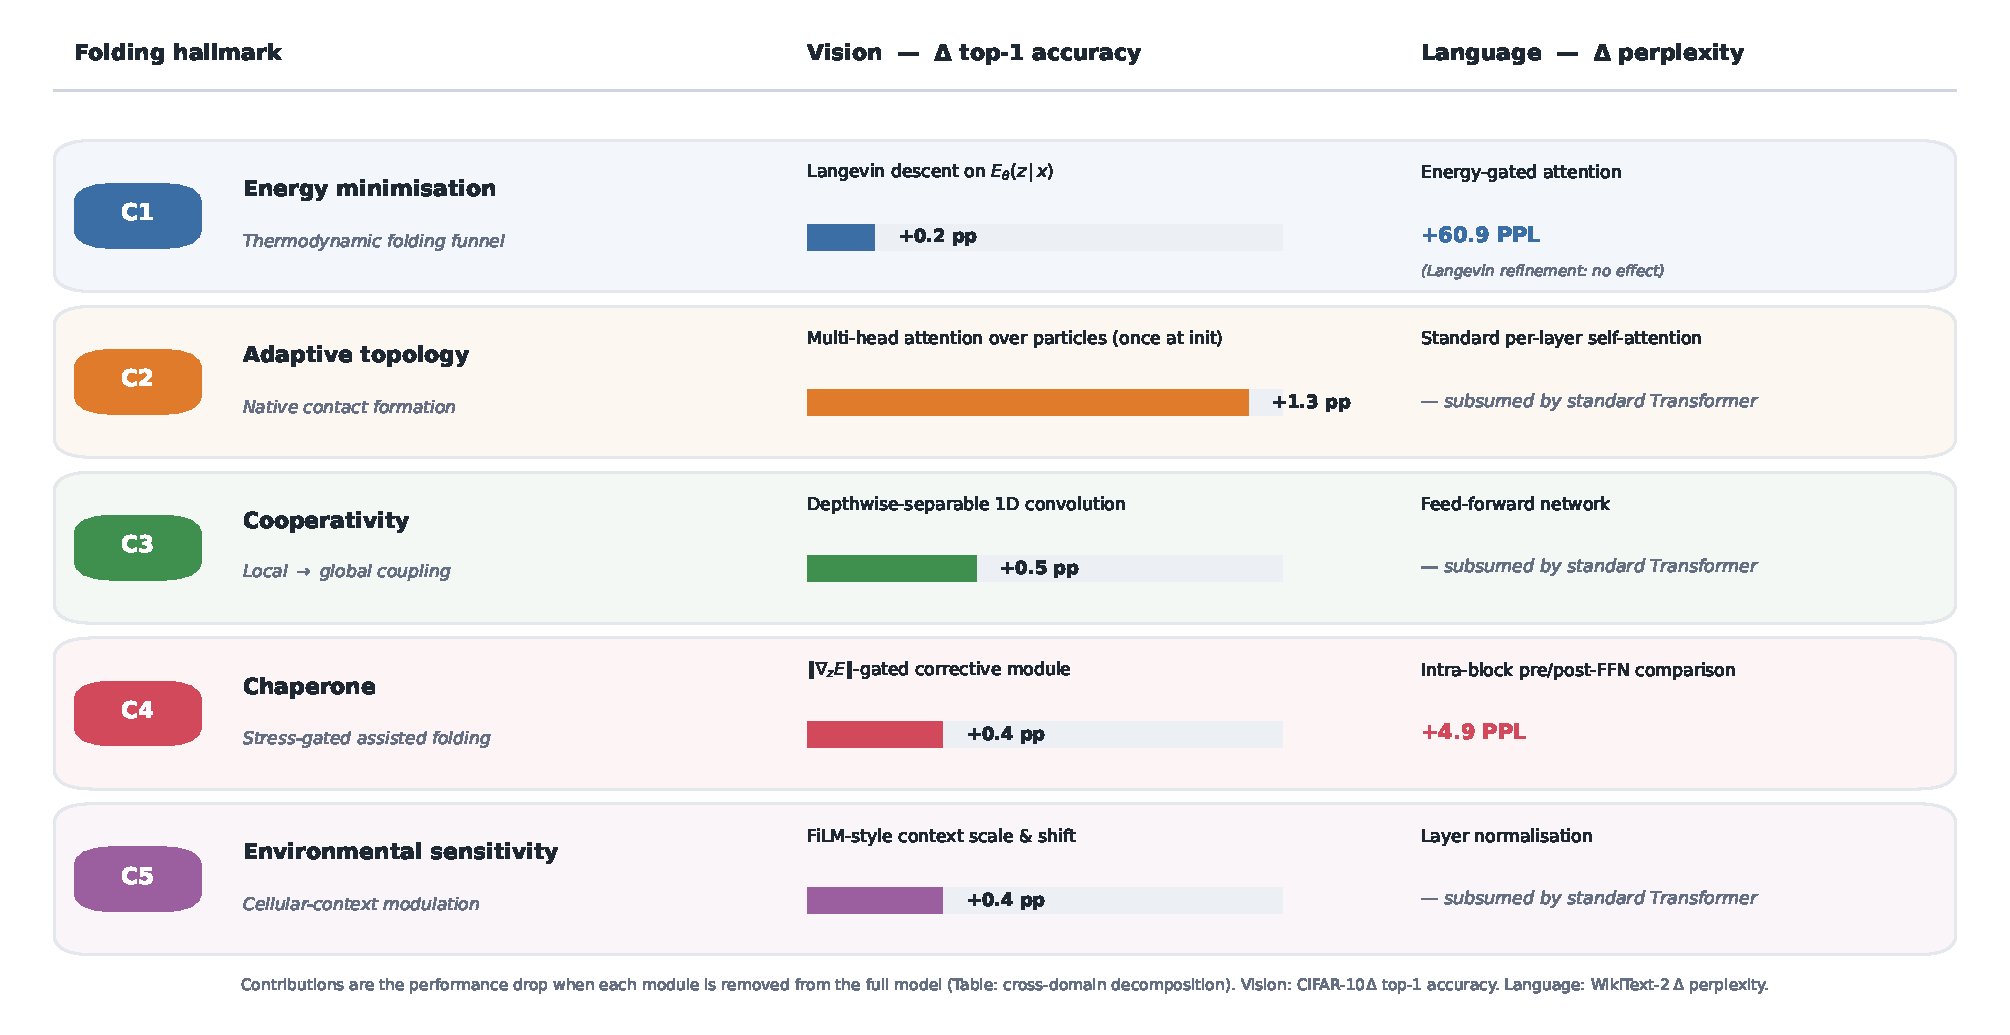
\includegraphics[width=\linewidth]{figures/fig_modules_detail.pdf}
  \caption{\textbf{Per-principle module reference.} For each of the
  five protein-folding hallmarks (C1--C5): its biological motivation,
  its vision and language instantiations, and its measured
  contribution---the change in CIFAR-10 top-1 accuracy (vision) and
  WikiText-2 perplexity (language) when that module is removed from
  the full model. The same principle is realised differently across
  modalities---e.g.\ energy minimisation (C1) is Langevin refinement
  in vision but energy-gated attention in language---while
  cooperativity (C3), environmental sensitivity (C5) and, in language,
  adaptive topology (C2) are subsumed by standard Transformer
  components. Values are taken from Table~\ref{tab:cross_domain}.}
  \label{fig:modules}
\end{figure}

The pattern is consistent with the biological metaphor: protein
folding is a multi-mechanism process in which different forces
dominate at different stages and for different substrates. For
autoregressive language generation, the dominant benefit comes from
context-dependent modulation of information flow (energy gating
mirrors energy-dependent contact strength). For image
classification, the dominant benefit comes from structural
reorganisation (adaptive topology mirrors native contact map
formation). Only a decomposed, modality-specific evaluation reveals
this pattern.

% ====================================================================
\section*{Discussion}
\label{sec:discussion}

Our results support three conclusions of direct interest to the
machine-learning community and to researchers interested in
bio-inspired computation more broadly.

\paragraph{Folding principles are useful inductive biases, but only some transfer.}
All five folding principles improved CIFAR-10 accuracy
incrementally, and in combination they produced a statistically
significant but small $+1.4$~pp gain over the baseline (83.0\% at
50 epochs; 85.72\% at 200 epochs). For language modelling, three of
the principles---energy gating, chaperone and Langevin
refinement---were instantiated, yet only one of the three
produced a reliable post-fix benefit. Langevin refinement had
\emph{no effect} on WikiText-2 perplexity, despite being the most
physically central principle in the folding analogy. The
post-fix $4.1\%$ perplexity reduction over the Transformer++
baseline (Table~\ref{tab:lm_attn_variants}) is small but reliable
across 5 seeds and survives a per-token causal control that is
agnostic to the energy framing. \emph{An earlier version of this
paper reported a $14.4\%$ reduction under a non-causal cumulative-mean
gate that read future tokens during teacher forcing; we trace that
result to a single line of code, replace the gate with a causal
cumulative mean, and report the corrected $4.1\%$ figure
transparently. The structural narrative survives the correction;
the magnitude is the part that shifts.} The honest conclusion
remains modality-dependent: useful folding-inspired modules exist,
but which principle helps depends on the task. This argues against
wholesale adoption of bio-inspired architectures and
for principle-by-principle evaluation.

\paragraph{Why does energy gating help so much in language?}
Energy-gated attention (Methods, Eq.~\ref{eq:energy_gate}) modulates
each attention head's contribution based on a global energy signal.
This is mathematically reminiscent of sparse mixture-of-experts
routing at the head level,\cite{shazeer2017outrageously,fedus2022switch}
but with two key differences: the gates are derived from a
mean-field energy function rather than a learned router, providing a
smooth and interpretable modulation, and all heads remain active
(soft gating) rather than being discretely selected, avoiding the
load-balancing issues of sparse MoE. The biological analogy is direct:
in folding, the strength of residue--residue contacts depends on the
overall energy state of the chain, with favourable contacts
strengthening as energy decreases.\cite{dill2012protein} Energy-gated
attention mirrors this by modulating head contribution based on the
``energy state'' (mean hidden representation) of the sequence.

\paragraph{Relation to head-level gating literature.}
Our energy-gated attention sits within a well-established head-gating
lineage that we should position explicitly. \emph{Talking-Heads
attention}\cite{shazeer2020talkingheads} learns linear projections
across the head dimension both before and after the softmax,
implementing a head-mixing mechanism. \emph{Squeeze-and-Excitation
networks}\cite{hu2018squeeze} popularised channel-wise gating in
vision, with sigmoid gates derived from a global average pool ---
structurally identical to our gate, swapping channels for heads.
\emph{Head-pruning analyses}\cite{voita2019analyzing,michel2019sixteen}
demonstrated that many transformer heads are redundant, so any
gating mechanism that softly de-weights uninformative heads should
help. Energy-gated attention is therefore a head-level,
context-dependent, sigmoid-gated soft-selection mechanism --- a known
design pattern with an energy-derived (rather than channel- or
projection-derived) gating signal. We frame this honestly: the
energy framing is an \emph{interpretation} of a known design
pattern, and our empirical contribution is the modality-dependent
ablation evidence rather than a novel gating mechanism.

\paragraph{Relation to topology-aware vision transformers.}
The C2 ``adaptive topology'' module is conceptually adjacent to a
topology-aware vision-transformer line.
\emph{Hypergraph Transformers (HGFormer)}\cite{hgformer2022} encode
multi-way connectivity in attention masks; \emph{Focal
Transformers}\cite{focal2021} inject locality biases into the
attention pattern; \emph{ConViT}\cite{dascoli2021convit} more generally
incorporates inductive biases into ViT attention. C2 differs from
all three in that the attention update is applied \emph{once} at
particle initialisation and the resulting feature update is then
propagated through the dynamics, rather than the attention pattern
being re-applied at every layer. This single-application design is
motivated by the protein-folding analogy (native contact map is
largely determined by sequence, not recomputed during folding) but
the reader who is sceptical of that motivation can equivalently
read C2 as a one-time inductive-bias injection in the spirit of
those prior works.

\paragraph{Why does Langevin refinement not transfer to language modelling?}
With converged training, both pre-fix and post-fix sweeps find
that Langevin refinement adds nothing measurable on WikiText-2
(pre-fix: full and ``w/o Langevin'' both at $512.5$~PPL; post-fix
sweep: Causal Energy and per-token causal gates differ from the
no-gate Transformer++ baseline by similar amounts whether or not
the dynamics include Langevin steps). We
hypothesise two factors. First, the energy head that drives Langevin
refinement receives only weak gradient signal in the autoregressive
setting, because the refinement acts on the final hidden state and
the loss is a standard token-level cross-entropy. Second, the
detach-and-reattach loop used to compute gradients through the
dynamics truncates gradient flow, preventing the energy head from
learning useful refinement directions. In the vision setting,
Langevin operates on a shared particle set with pooled readout,
which is more tolerant of per-step noise and provides a clearer
energy landscape for refinement. Designing score-matching training
objectives\cite{song2019generative} or learning the energy head on
an auxiliary denoising task are natural directions for reviving this
component in language modelling.

\paragraph{Relation to feature-wise modulation.}
The environmental-sensitivity module (C5) is closely related to
Feature-wise Linear Modulation (FiLM),\cite{perez2018film} which
applies learned affine transformations conditioned on an auxiliary
input. Our variant differs in that the conditioning signal $\bc$ is
derived from the same input encoder (rather than a separate
modality) and uses a Softplus-shifted scale to ensure stability
during Langevin dynamics. The broader principle of
context-dependent scale-and-shift is shared, and FoldFlow should be
read as an ablation \emph{of} FiLM-style modulation in the specific
context of folding-inspired dynamics rather than as a novel
conditioning mechanism.

\paragraph{Limitations and scope.}
The evaluation uses CIFAR-10 and WikiText-2, benchmarks chosen to
isolate architectural contributions at modest cost; generalisation
to ImageNet and large language corpora remains to be established.
Langevin dynamics add sequential computation ($T{=}8$ steps for
classification, $K{=}3$ for language-model inference), which
increases wall-clock inference latency relative to purely
feed-forward models, although our observed training throughput is
competitive. The energy function in C1 is a learned mean-field MLP
and therefore does not literally capture pairwise residue
interactions as in physical protein energy functions; exploring
pairwise or attention-based energy parameterisations is a natural
next step. Finally, our two-modality evaluation by construction
cannot address generalisation to structured-prediction tasks,
reinforcement learning or multimodal problems; we view FoldFlow as
an architectural template whose principles we expect to transfer
selectively across modalities, exactly as the folding metaphor
predicts.

\paragraph{Broader impact.}
This work explores bio-inspired inductive biases for neural
architecture design. The principles studied (energy minimisation,
topology, cooperativity, chaperone correction, environmental
sensitivity) are general-purpose and do not raise specific ethical
concerns beyond those common to neural-network research. The
computational cost of our experiments is modest (single-device
training on an Apple M-series chip); all code and configurations
will be released to support reproducibility. We encourage the
community to treat folding as one concrete instance of a broader
programme of principled extraction of inductive biases from
biological self-assembly processes, with rigorous modality-level
evaluation of which mechanisms improve which tasks.

% ====================================================================
\section*{Methods}
\label{sec:methods}

\subsection*{Latent particles and encoder}

Given an input $\bx$ (an image or a sequence of token embeddings),
a learned encoder maps $\bx$ to a context vector $\bc \in \R^{H}$,
which is used both to initialise the particles and to condition
every FoldFlow module. Particles
$\bz^{(0)} \in \R^{N \times D}$ are produced by a linear projection
of $\bc$ and a learned positional embedding. For CIFAR-10 we use
$N=64$ particles of dimension $D=64$; for WikiText-2 we skip the
particle-set construction and operate directly on the hidden states
of a 6-layer, 8-head Transformer with $d_\text{model}=512$.

\subsection*{C1: Energy minimisation via Langevin dynamics}

We define a learnable energy function
$\E_{\btheta} : \R^{N \times D} \times \R^{H} \to \R$ conditioned on
the encoder context $\bc$:
\begin{equation}
  \E_{\btheta}(\bz, \bc) = \sum_{i=1}^{N}
    f_{\btheta}\left([\bz_i; \bc]\right),
\label{eq:energy}
\end{equation}
where $f_{\btheta}$ is a three-layer MLP. Particles evolve by
discretised Langevin dynamics with a learned, input-adaptive step
size $\epsilon(\bc)$:
\begin{equation}
  \bz^{(t+1)} = \bz^{(t)}
    - \epsilon(\bc) \, \tau_t \, \grad_{\bz} \E_{\btheta}(\bz^{(t)}, \bc)
    + \sqrt{2\tau_t}\,\sigma\,\boldsymbol{\eta},
  \qquad \boldsymbol{\eta} \sim \mathcal{N}(0, \mathbf{I}),
\label{eq:langevin}
\end{equation}
where $\tau_t$ is annealed linearly from 1.0 to 0.1 over $T$ steps
and $\sigma = 0.01$ controls noise magnitude. Physically, this is a
temperature-annealed gradient descent on a learned landscape: at
early steps the noise facilitates broad exploration, while at late steps
the dynamics approach the minimum of $\E_{\btheta}$.

\subsection*{C2: Adaptive topology}

We model the input-dependent connectivity between particles with a
multi-head self-attention operation, computed \emph{once} after
initialisation (Algorithm~\ref{alg:foldflow}, line 3):
\begin{equation}
  \bz \leftarrow \bz + \text{MHA}(\text{LN}(\bz)).
\end{equation}
The learned topology is then fixed for the duration of the
Langevin dynamics. This choice, corrected from an earlier
``dynamic topology'' description, mirrors the empirical finding that
a protein's native contact map is primarily determined by its
sequence, and is not recomputed at every folding step.

\subsection*{C3: Cooperativity}

Local secondary structure in folding stabilises long-range tertiary
contacts. We instantiate this with a depthwise-separable 1D
convolution over the particle sequence:
\begin{equation}
  \bz \leftarrow \bz + \alpha \cdot \text{PWConv}(\text{DWConv}(\text{LN}(\bz))),
\end{equation}
where $\alpha$ is a learnable scale initialised to 0.1, and the
module is applied at every dynamics step before the energy
gradient.

\subsection*{C4: Stress-gated chaperone}

We measure ``folding stress'' as the mean gradient norm
$s = \frac{1}{N}\sum_i \|\grad_{\bz_i} \E\|$ and gate a corrective
network accordingly:
\begin{equation}
  \bz \leftarrow \bz + \alpha \cdot \sigma(s) \cdot
    g_{\btheta}\!\left([\bar{\bz}; \bc; \sigma(s)]\right),
\end{equation}
where $\bar{\bz} = \frac{1}{N}\sum_i \bz_i$, $\sigma(\cdot)$ is the
sigmoid function, and $g_{\btheta}$ is a two-layer MLP with Tanh output.
The chaperone intervenes every other dynamics step, mirroring the
biological observation that chaperones engage only when folding
intermediates are under stress.\cite{hartl2011molecular}

\subsection*{C5: Environmental sensitivity}

We model cellular-context dependence as a FiLM-style\cite{perez2018film}
affine modulation:
\begin{equation}
  \bz \leftarrow (\gamma(\bc) + 0.5) \odot \bz + \beta(\bc),
\end{equation}
where $\gamma$ uses a Softplus activation to ensure a strictly
positive scale. This is applied at particle initialisation and
every third dynamics step. The Softplus-shifted scale and the
derivation of $\bc$ from the primary encoder (rather than a
separate modality) are the main differences from the original FiLM
formulation.

\subsection*{Readout}

After $T$ dynamics steps, particle states are mean-pooled and
projected through a two-layer MLP to produce the final prediction.
No skip connection from the encoder to the readout is used,
ensuring that all discriminative information flows through the
particle dynamics. Algorithm~\ref{alg:foldflow} summarises the full
vision pipeline.

\begin{algorithm}[t]
\caption{FoldFlow particle dynamics (vision).}\label{alg:foldflow}
\begin{algorithmic}[1]
\REQUIRE Input $\bx$, dynamics steps $T$, energy $\E_{\btheta}$
\STATE $\bc \leftarrow \text{Encoder}(\bx)$
\STATE $\bz^{(0)} \leftarrow \text{InitParticles}(\bc)$
\STATE $\bz^{(0)} \leftarrow \bz^{(0)} + \text{MHA}(\text{LN}(\bz^{(0)}))$ \COMMENT{C2, applied once}
\STATE $\bz^{(0)} \leftarrow (\gamma(\bc)+0.5) \odot \bz^{(0)} + \beta(\bc)$ \COMMENT{C5: init}
\FOR{$t = 0$ \TO $T-1$}
  \STATE $\bz \leftarrow \bz + \alpha \cdot \text{PWConv}(\text{DWConv}(\text{LN}(\bz)))$ \COMMENT{C3}
  \STATE $\tau_t \leftarrow 1.0 - 0.9 \cdot t / T$
  \STATE $\bz \leftarrow \bz - \epsilon(\bc)\tau_t \grad_{\bz} \E_{\btheta}(\bz, \bc) + \sqrt{2\tau_t}\sigma \boldsymbol{\eta}$ \COMMENT{C1}
  \IF{$t \bmod 2 = 0$}
    \STATE $s \leftarrow \tfrac{1}{N}\sum_i \|\grad_{\bz_i}\E\|$; \quad $\bz \leftarrow \bz + \alpha\sigma(s) g_{\btheta}([\bar\bz; \bc; \sigma(s)])$ \COMMENT{C4}
  \ENDIF
  \IF{$t \bmod 3 = 0$}
    \STATE $\bz \leftarrow (\gamma(\bc)+0.5) \odot \bz + \beta(\bc)$ \COMMENT{C5}
  \ENDIF
\ENDFOR
\RETURN $\text{MLP}(\text{MeanPool}(\bz^{(T)}))$
\end{algorithmic}
\end{algorithm}

\subsection*{FoldFlow for language modelling}

To evaluate whether the folding principles generalise beyond
particle-based vision, we adapt three components for autoregressive
language modelling on top of a standard
Transformer.\cite{vaswani2017attention}

\paragraph{Causal energy-gated attention.}
In standard multi-head attention, all heads contribute equally. We
introduce per-position, per-head energy gates: at each position $t$,
a two-layer MLP over the \emph{causal cumulative mean} of the hidden
state produces $h$ sigmoid gates $\mathbf{g}_t \in [0,1]^h$, one per
head. Each head's attention output at position $t$ is scaled by its
gate before the output projection:
\begin{equation}
  \text{EnergyAttn}(\bx)_t = W_O \left[\, g_{t,1} \cdot \text{head}_1(\bx)_t \,;\, \ldots \,;\, g_{t,h} \cdot \text{head}_h(\bx)_t \,\right],
\label{eq:energy_gate}
\end{equation}
\begin{equation}
  g_{t,i} = \sigma\!\left(\text{MLP}(\bar\bx_{\le t})\right)_i,
  \qquad \bar\bx_{\le t} = \frac{1}{t+1} \sum_{s = 0}^{t} \bx_s.
\label{eq:causal_ctx}
\end{equation}
The cumulative-mean context $\bar\bx_{\le t}$ depends only on tokens
at positions $\le t$, so the gate is causal by construction:
$\partial g_{t,i} / \partial \bx_{t'} = 0$ for all $t' > t$. We
verify this empirically by gradient inspection across all three
attention variants we evaluate (Causal energy gating, per-token
causal, and Talking-Heads); see ``Causal energy gating''
below for the verification protocol. The biological reading remains
that of soft head selection,\cite{shazeer2017outrageously} with the
gating signal derived from an energy-inspired context function
rather than a learned router; the correction restricts that context
to the strictly causal past.

\paragraph{Intra-block chaperone correction.}
Each FoldFlow-LM block compares pre- and post-feed-forward hidden
states and produces a scaled corrective signal:
\begin{equation}
  \bx_\text{out} = \bx_\text{ffn} + \alpha_\text{chap} \cdot
  \text{Tanh}\!\left(W_2 \,\text{GELU}(W_1 [\bx_\text{pre};\, \bx_\text{ffn}])\right),
\end{equation}
where $\alpha_\text{chap}$ is a learnable scalar initialised to 0.1.

\paragraph{Langevin refinement.}
After the final block, hidden states undergo $K$ gradient-descent
steps on a learned energy head
$E_\text{head}: \R^d \to \R$:
$\bz \leftarrow \bz - \epsilon \cdot \grad_{\bz} E_\text{head}(\bz)$,
with $K{=}3$ and $\epsilon{=}0.01$. The energy head is trained
end-to-end with the main cross-entropy loss.

\paragraph{Causal energy gating.}
An earlier formulation of Eq.~\ref{eq:energy_gate} pooled the
context globally, $\bar\bx = \tfrac{1}{L}\sum_{s=0}^{L-1}\bx_s$, so
that under teacher forcing the gate at every position read every
token of the same training sequence---including positions strictly
in the future. Although the multi-head attention itself is masked,
the per-head \emph{gate} multiplies the attention output and is
itself a function of $\bar\bx$, so $\partial g_i / \partial
\bx_{t'} \ne 0$ for $t' > t$. This breaks autoregressive causality
during training. We replace the global mean by the causal cumulative
mean of Eq.~\ref{eq:causal_ctx}, which preserves the per-head
gating mechanism while restricting the gate's input at position $t$
to tokens $\{\bx_0, \ldots, \bx_t\}$. We verify causality by a
gradient test: for randomly initialised models in each of the three
attention variants we evaluate (Causal energy gating, per-token
causal, Talking-Heads), we compute
$\| \partial \mathcal{L}_t / \partial \bx_{t'} \|$ for $t'>t$ and
confirm exact zero across positions. We additionally report a
re-estimate of the WikiText-2 perplexity gap under the corrected
gate (Table~\ref{tab:lm_attn_variants}) so that the headline
improvement number reflects the causally safe formulation.

\paragraph{Per-token causal gate and Talking-Heads baselines.}
To isolate which property of the energy gate matters, we evaluate
two ablations sharing the same backbone, parameter count and
training schedule. (a)~\emph{Per-token causal gate}: the gate at
position $t$ is computed from $\bx_t$ alone (no temporal pooling),
testing whether the cumulative-mean structure adds anything over
the simplest causal alternative. (b)~\emph{Talking-Heads
attention},\cite{shazeer2020talkingheads} which inserts a learned
linear projection across heads pre- and post-softmax---a well-known
head-mixing baseline that the gating literature
treats as the natural control. These directly probe whether
\emph{any} head-level reweighting matters versus the specific
energy-derived signal.

\paragraph{Baseline: Transformer++.}
The baseline uses the identical architecture skeleton---pre-norm
blocks,\cite{ba2016layer} GELU activation, tied embeddings and
identical hyperparameters---without energy gating, chaperone
correction, or Langevin refinement. This ensures that any
performance difference is attributable to the FoldFlow components
rather than configuration choices.

\subsection*{Experimental protocol}

All experiments were conducted on a single Apple M-series chip using
the Metal Performance Shaders (MPS) backend of
PyTorch. CIFAR-10 ablations use 3 seeds (42, 43, 44) over 50
epochs; the extended-training run uses 200 epochs. CIFAR-100 uses 3
seeds over 50 epochs. WikiText-2 uses 5 seeds (42--46), trains for up
to 17 epochs with early stopping, and selects the best-validation
epoch (typically 6--7). All models use AdamW with standard weight
decay (0.05 for vision, 0.01 for language), gradient clipping at
1.0, and cosine learning-rate decay with warmup. Full hyperparameter
tables and per-seed results are provided in the Supplementary
Material. Statistical comparisons use paired t-tests across seeds.

% ====================================================================
\section*{Data Availability}
\label{sec:data}
All datasets used in this study are publicly available standard
benchmarks. CIFAR-10 and CIFAR-100 are available from the University
of Toronto at \url{https://www.cs.toronto.edu/~kriz/cifar.html} and
via the Hugging Face datasets distribution.\cite{krizhevsky2009cifar}
WikiText-2~\cite{merity2017pointer} is available via the Hugging Face
datasets repository at \url{https://huggingface.co/datasets/Salesforce/wikitext}.
No new experimental data were generated during this study.
Pre-processing scripts, tokenisation details (GPT-2 tokeniser,
50{,}257 tokens), per-seed numerical results, training
configurations, and model checkpoints required to reproduce all
reported figures and tables are released in the FoldFlow repository:
\url{https://github.com/karimmagdy/FoldFlow}.

\section*{Code Availability}
\label{sec:code}
All code for training, evaluation and figure generation is
available at \url{https://github.com/karimmagdy/FoldFlow}, together
with exact seeds, configuration files, logs, and model checkpoints
sufficient to reproduce every table and figure in this paper. A
permanently archived snapshot of the exact code version used for
this study (GitHub release v1.0.0) is deposited in the Zenodo
repository under a citable DOI:
\href{https://doi.org/10.5281/zenodo.20932167}{10.5281/zenodo.20932167}.
Experiments were
run on a 2024 Apple M4 Mac (Apple silicon, MPS backend); the
codebase is also compatible with CUDA and has been spot-tested on
Google Colab Pro with A100/H100 GPUs. The full 70-hour experimental
budget is reported in the Supplementary Material.

% ====================================================================
\section*{References}
\renewcommand{\refname}{}
\vspace{-2em}
\bibliographystyle{plainnat}
\bibliography{references}

% ====================================================================
\section*{Acknowledgements}
We thank colleagues at the Arab Open University (Egypt) for
feedback and discussion. We also acknowledge the broader research
community for the open-source tools and datasets (PyTorch, Hugging
Face, CIFAR, WikiText) on which this work depends. Computational
resources were provided by the authors on personal hardware (Apple
M4) and by Google Colab Pro.

\section*{Funding}
The authors received no specific grant from any funding agency in the
public, commercial, or not-for-profit sectors for this work. Compute
resources (Google Colab Pro and personal hardware) were self-funded
by the corresponding author.

\section*{Author Contributions}
K.M.\ conceived the study, designed the FoldFlow architecture,
implemented the code, ran all experiments, analysed the data, and
drafted the manuscript. G.K.\ supervised the project, advised on
experimental design and interpretation, and contributed to
manuscript revisions. H.A.\ advised on statistical methodology and
on the protein-folding motivation, and contributed to manuscript
revisions. All authors read and approved the final manuscript.

\section*{Competing Interests}
The authors declare no competing interests.

\section*{Additional Information}
Supplementary Information accompanies this paper. Correspondence
and requests for materials should be addressed to K.M.

\end{document}
